\documentclass[11pt,letterpaper]{article}

% Load package
\usepackage{lesson}
\usepackage{amsmath}
\usepackage{xcolor}
\usepackage{url}

%--------------------------------------%
% Custom commands include:             %
%%%%%%%%%%%%%%%%%%%%%%%%%%%%%%%%%%%%%%%%
% Include an image:                    %
% \diagram{height}{align}{file}        %
%                                      %
% height: a number representing mm     %
% align: left, center, or right        %
% file: file name without extension    %
%%%%%%%%%%%%%%%%%%%%%%%%%%%%%%%%%%%%%%%%
% Add a numbered question:             %
% \question{text}                      %
% \questiond[lines]{file}{width}{text} %
%                                      %
% lines: # of lines of text to wrap    %
% file: file name without extension    %
% width: a % of textwidth for image    %
%%%%%%%%%%%%%%%%%%%%%%%%%%%%%%%%%%%%%%%%
% Add a lettered option/question part: %
% \option[vspace]{text}                %
%                                      %
% vspace: added space above the option %
%%%%%%%%%%%%%%%%%%%%%%%%%%%%%%%%%%%%%%%%
% Add a blank line in text:            %
% \blankline{width}                    %
%%%%%%%%%%%%%%%%%%%%%%%%%%%%%%%%%%%%%%%%
% Add an arc symbol in math:           %
% \arc{notation}                       %
%--------------------------------------%
%%%%%%%%%%%%%%%%%%%%%%%%%%%%%%%%%%%%%%%%
%--------------------------------------%
% To reset the question counter:       %
% \setcounter{qcounter}{0}             %
%                                      %
% To reset the option counter:         %
% \setcounter{acounter}{0}             %
%--------------------------------------%

% Set title and course name
\settitle{Week 3 Question Set}
\setsubtitle{Synapses, dendrites and cable equation \& Machinery of Vision}
\setcourse{Summer 2023}

\begin{document}

% Create title and add proper header for first page
\maketitle
\thispagestyle{first}

\section{CNS3.1 - Synapses}
\begin{enumerate}
    \item For each of the listed neurotransmitter receptors, identify their characteristics by filling in the table below:
    \begin{table}[h]
        \centering
        \begin{tabular}{|c|c|c|c|}
            \hline
            Receptor & Excitatory or Inhibitory? & Fast or Slow Action? & Causes influx or efflux of what ion?\\
            \hline
            \hline
            AMPA & & &\\
            \hline
            NMDA & & &\\
            \hline
            GABA$_A$ & & &\\
            \hline
            GABA$_B$ & & &\\
        \hline
        \end{tabular}
    \end{table}

    \item Let's dissect this equation that represent the conductance of a synapse:
    \begin{align*}
        g_{syn} (t) = \sum_k \bar{g}_{syn} \, e^{-(t-t_k)/\tau} \left[ 1 - e^{-(t-t_k)/\tau_{rise}} \right] \Theta (t - t_k)
    \end{align*}
    Each term in the equation plays a significant role in representing synaptic conductance. Can you match each term to its appropriate description?
    \begin{itemize}
        \item Terms: 
        \begin{enumerate}
            \item[i.] $\Theta (t - t_k)$
            \item[ii.] $\bar{g}_{syn}$
            \item[iii.] $1 - e^{-(t-t_k)/\tau_{rise}}$
            \item[iv.] $e^{-(t-t_k)/\tau}$
        \end{enumerate}
    \end{itemize}
    \begin{itemize}
        \item Descriptions: 
        \begin{enumerate}
            \item This is the synaptic conductance of a single presynaptic action potential.
            \item This models the rise of conductance, avoiding an unrealistic instantaneous increase.
            \item This is the Heaviside step function, ensuring all values before $t_k$ equal zero.
            \item This term models the exponential decay of synaptic conductance, representing the gradual restoration of the electrical gradient.
        \end{enumerate}
    \end{itemize}

    \pagebreak

    \item How does GABA$_A$ receptor activation lead to shunting inhibition in a neuron?
    \begin{enumerate}
        \item [a.] It allows sodium ions to flow into the cell, depolarizing the neuron.
        \item [b.] It allows potassium ions to flow out of the cell, hyperpolarizing the neuron.
        \item [c.] It allows chloride ions to flow into the cell, maintaining the membrane potential closer to the resting state and reducing the effect of excitatory signals.
        \item [d.] It prevents calcium ions from flowing into the cell, stopping the propagation of the action potential.
    \end{enumerate}

    
    \end{enumerate}
\pagebreak

\section{CNS3.2 - Synaptic Short Term Plasticity}
\begin{enumerate}
    \item The lecture introduce a new quantity called Fraction of Filled Released Sites ($P_{rel}$) with the following formula by Dayan and Abbott, 2001:
    \begin{align*}
        \frac{d P_{rel}}{dt} = -\frac{P_{rel} - P_0}{\tau_P} - f_D P_{rel} \, \sum_k \delta(t - t^k)
    \end{align*}
    Dissect this equation and match each term with the correct description:
    \begin{itemize}
        \item Terms: 
        \begin{enumerate}
            \item[i.] $\frac{P_{rel} - P_0}{\tau_P}$
            \item[ii.] $f_D P_{rel}$
            \item[iii.] $\delta(t - t^k)$
        \end{enumerate}
    \end{itemize}
    \begin{itemize}
        \item Descriptions: 
        \begin{enumerate}
            \item This term represents the amount of neurotransmitter released (and thereby becoming unavailable) at this instant of time.
            \item This gives rise to the exponential decay / restoration of $P_{rel} (t)$ to the steadystate level $P_0$.
            \item This contributes to the instantaneous changes in $P_{rel} (t)$ at the moments of presynaptic firing.
        \end{enumerate}
    \end{itemize}

    \item Based on the previous descriptions, what is the most probable shape of the solution $P_{rel}(t)$ to the given differential equation?
    \begin{enumerate}
        \item A sum of shifted exponential saturations, converging to a steady-state value.
        \item A sum of sinusoidal waves, oscillating between a minimum and maximum value.
        \item A sum of shifted exponential decays, converging to a steady-state value.
        \item A series of step functions, abruptly changing at specific times.
        \item A combination of stepwise reductions and exponential recoveries.
    \end{enumerate}

\end{enumerate}


\pagebreak

\section{CNS3.3 - Dendrite as a Cable and Cable Equation}
\begin{enumerate}
    \item The lecture mentions that the numerical approximation for the second derivative of a function can be expressed as:
    \begin{align*}
        f''(t) \approx \frac{f(t-dt) - 2f(t) + f(t+dt)}{(dt)^2}
    \end{align*} Let's walk through the steps to derive this approximation.
    \begin{enumerate}
        \item First, apply the Taylor expansion to the expressions $f(t-dt)$ and $f(t+dt)$. Remember that the Taylor expansion for a function around a point $t$ is:
        \begin{align*}
            f(t + dt) = f(t) + dt \cdot f'(t) + \frac{(dt)^2}{2!} \cdot f''(t) + \frac{(dt)^3}{3!} \cdot f'''(t) + \cdots + \frac{(dt)^n}{n!} \cdot f^{(n)}(t) + O(dt^{n+1})
        \end{align*}
        \vspace{2 cm}
        \item Next, combine these two expansions by adding $f(t-dt)$ and $f(t+dt)$, then isolate $f''(t)$ in the resulting equation.
        \vspace{5 cm}
        \item Finally, assume that the step size $dt$ is sufficiently small, so the error term $O((dt)^3)$ and beyond can be removed. This will give you the approximation for $f''(t)$.
        \vspace{2 cm}
    \end{enumerate}

    \item Which of the following factors contribute to the longitudinal resistance ($R_L$, not the per unit length variable $r_L$) in a neuron's axon or dendrite? (Choose all that apply)
    \begin{enumerate}
        \item The resistivity of the intracellular medium
        \item The cross-sectional area of the neuronal structure
        \item The length of the axon or dendrite
        \item The concentration of extracellular ions
    \end{enumerate}
\end{enumerate}

\pagebreak


\section{CNS3.4 - Cable equation}
\begin{enumerate}
    \item 
    The cable equation, which describes the behavior of electrical potential in neuronal dendrites and axons, is given as:
    % \begin{equation}
    % \frac{\partial^2 u(t, x)}{\partial x^2} = c , r_L \frac{\partial u(t, x)}{\partial t} + r_L \sum_{\text{ion}} i_{\text{ion}} (t, x) - r_L i^{\text{ext}} (t, x)
    % \end{equation},
    % where $r_L$ is the longitudinal resistance (per unit length), $c$ is the membrane capacitance (per unit length), $i^{\text{ext}}$ and $i_{\text{ion}}$ represent the external and ionic currents (both per unit length), respectively, and $u(t, x)$ is the membrane potential (per unit length).
    \begin{equation}
        \lambda^2 \frac{\partial^2 u(t, x)}{\partial x^2} = \tau_m \frac{\partial u(t, x)}{\partial t} + u(t, x) - r_m \, i^{ext} (t, x),
    \end{equation}
    where $\lambda = \sqrt{r_m / r_i}$ is the space constant, $\tau_m = c \cdot r_m$ is the time constant, $i^{\text{ext}}$ represent the external currents, and $u(t, x)$ is the membrane potential. Everything lower-case are per unit length.
    \begin{center}
    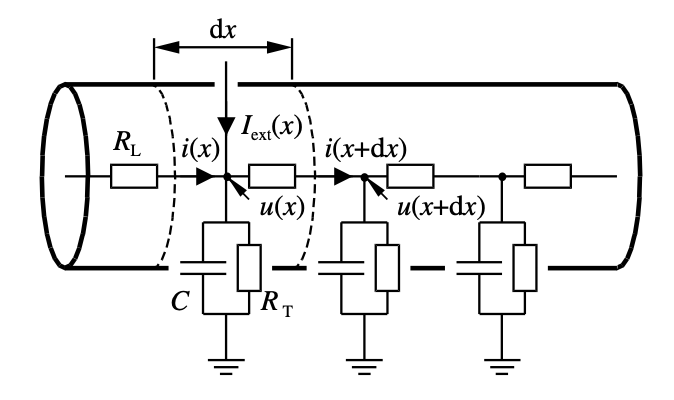
\includegraphics[scale=0.5]{4.1.png}
    \end{center}
    
    Interestingly, this bears a resemblance to the heat equation:
    \begin{equation}
    \alpha \frac{\partial^2 u(t, x)}{\partial x^2} = \frac{\partial u(t, x)}{\partial t}
    \end{equation}
    In this equation, $u$ represents the temperature, $t$ is the time, $x$ is the position in the medium, and $\alpha$ is the thermal diffusivity of the medium. The heat equation tells us how heat diffuses through a medium over time. To learn more about heat equation, please watch this video by 3Blue1Brown: \url{https://youtu.be/ly4S0oi3Yz8}. 
    
    \begin{enumerate}
        \item Can you articulate why these two equations seem similar in form? \emph{Hint}: Is there anything also "diffusing" over space and time in the cable?

        \vspace{3 cm}

        \item The space constant $\lambda$ describes how far along a cable-like structure (such as an axon or dendrite) a graded potential can travel before decaying to a certain percentage of its original amplitude. What is this percentage?
        \begin{enumerate}
            \item 10\%
            \item 25\%
            \item 37\%
            \item 50\%
        \end{enumerate}
    \end{enumerate}

\end{enumerate}


\pagebreak

\section{CNS3.5 - Compartmental Models}
\begin{enumerate}
    \item The compartmental modeling approach is often used to numerically solve the cable equation for complex dendritic trees. Which of the following statements is correct regarding this approach?
    \begin{enumerate}
        \item The dendritic tree is divided into small cylindrical compartments with uniform membrane potential, each characterized by its capacity and transversal conductivity. 
        \item Numerical methods transform the cable equation into a system of ordinary differential equations that can be solved for the membrane potential at various discretization points over time.
        \item Nonlinear ion channels, responsible for generating spikes, are typically grouped together at the soma while treating the dendritic tree as a passive cable.
        \item All of the above.
    \end{enumerate}

    \item Which of the following statements about back-propagating action potentials is correct?
    \begin{enumerate}
        \item Back-propagating action potentials are directly related to the backpropagation algorithm used in neural networks.
        \item Back-propagating action potentials travel from the soma towards the dendrites.
        \item Back-propagating action potentials serve no functional purpose in a neuron and are only observed during artificial stimulation.
        \item Back-propagating action potentials have a role in synaptic plasticity and can modulate the strength of synapses based on their timing relative to forward-propagating action potentials.
    \end{enumerate}


\end{enumerate}

\pagebreak

\section{V\&B Chapter 3 - The Neuronal Machinery of Vision}
\begin{enumerate}
    \item  In the context of neuronal signaling, what biological mechanism or structure serves a similar function to a 'signal booster' in an axon?

    \vspace{2 cm}

    \item The author has referenced several key figures in the field of visual neuroscience, each of whom made significant discoveries about the retina using different animal models. Please fill in the table below with the specific animals they used and their corresponding findings.
    \begin{table}[h]
        \centering
        \begin{tabular}{c|c|c|c}
            Scientist's Name & Year of Discovery & Animal Model Used & Key Findings about the Retina \\
            \hline
            \hline
            H. Keffer Hartline & 1949 & &\\
            \hline
            Horace Barlow & 1953 & & \\
            \hline
            Stephen Kuffler & 1953 & &\\
        \end{tabular}
    \end{table}

    \item Choose the \textbf{incorrect} statement related to the receptive field of retinal ganglion cells:
    \begin{enumerate}
        \item[a.] The term "receptive field" refers to the area of the sensory world that a neuron responds to.
        \item[b.] The center-surround structure of the receptive field ensures that the information sent to the brain highlights the absolute intensity at each point in the visual field.
        \item[c.] For ON-center cells, light in the center of the receptive field will increase the cell's firing rate.
        \item[d.] For OFF-center cells, light in the center decreases the firing rate, while light in the surround increases it.
    \end{enumerate}
    
    \item The receptive field's center-surround structure in vision resembles a 'Mexican hat'. In computer vision, the Mexican hat wavelet is used for edge detection as it approximates the Laplacian of Gaussian operator. When this operator is applied to an image through convolution, it effectively takes the second derivative of the image. Why would identifying the zero-crossing points be useful following the application of the Mexican hat wavelet to an image?

    \pagebreak
    
    \item Fourier analysis uses sinusoids for signal decomposition and composition. Which of the following statements about sinusoids is \textbf{incorrect}?
    \begin{enumerate}
        \item The use of sinusoids benefits from their orthogonality, meaning the dot product of two sinusoids of different frequencies or the same frequency but 180 degrees out of phase, is zero. This makes the representation highly efficient.
        \item Each sinusoid corresponds to a precise frequency, making them perfect for frequency analysis.
        \item Sinusoids assist in localizing the exact time or spatial location where a particular frequency occurs.
        \item The property of sinusoidal fidelity in linear systems signifies that these systems cannot create or destroy sinusoids, but only alter their amplitude or phase. This property makes them relatively easy to work with mathematically.
    \end{enumerate}

    \item Circle the correct option: From a computational perspective, one can consider the retina as a set of spatial (low-pass/high-pass/band-pass) filters performing Fourier decomposition on the retinal images.
    
    \item The author provides two reasons why both on-center and off-center cells exist. The first reason involves reducing the need for a high baseline firing rate. The second reason, which is more intricate, employs the analogy of push-pull amplifiers. Let's delve into the second reason:
    \begin{enumerate}
        \item The author claims: "Engineers worked out a long time ago that a linear amplifier can be made using nonlinear components provided the input signal is first split into a mostly negative and a mostly positive part...". Let's use a toy example to illustrate this. Suppose our goal is to construct a linear amplifier such that its output $g(x)$ scales linearly with the input $x$. However, we only have access to two nonlinear amplifiers: $f_1(x) = |x|$ and $f_2(x) = |-x|$. How would you combine $f_1(x)$ and $f_2(x)$ to yield a linear output $g(x) = 2x$?
    
        \vspace{3 cm}
    
        \item Following the previous question, can you perceive how the range of the cumulative output is now double that of any single neuron considered in isolation?
    
        \vspace{1.5 cm}
    
        \item The author notes that linearity simplifies the interpretation of outputs from a system, whether it's a neuron or an amplifier, making it a desirable characteristic in many cases. Nonetheless, there are instances where nonlinearity is indispensable. For example, neurons detecting motion exhibit robust responses when a bright spot travels across the visual field in their preferred direction, yet they show disproportionally little response when the spot moves slowly. In what way is this phenomenon nonlinear?
    
        \vspace{3 cm}
    \end{enumerate}


    \item According to Ben Logan's theorem (1977), we can transform from one representation to another. Fill in the blanks with the appropriate terms: 'luminance edges' and 'image'. The theorem suggests that we can transform from \underline{\hspace{4 cm}} to \underline{\hspace{4 cm}}, providing an efficient coding of the retinal image.

    \item Select the correct option: Under low-light conditions, retinal ganglion cells exhibit a Gaussian (bell-shaped) receptive field rather than a Mexican hat-like shape. This shift is because \underline{\hspace{2 cm}} operation aids in noise reduction.
    \begin{enumerate}
        \item Band-pass
        \item Averaging
    \end{enumerate}
    


    

\end{enumerate}

\end{document}